\section{Co-Design Aspects}
\color{red}
Co-design	aspects,	e.g.,	necesity for	re-design.	Your	design	decision	and	justification
\color{black}
While above sections describe formulating initial design that satisfy design constraints, this section deals with obtaining an optimal one. For this purpose an automated script is built to search through the search space for obtaining an optimal solution. Following observations are made from the experiments.

\begin{enumerate}
	\item TDM frame size is inversely proportional to QOC. This is because less are the number of slots allocated to application more is the delay between successive samplings. This makes the system to respond slowly i.e higher settling time and lesser control. On the contrary when more slots are allocated to the application the delay between successive samplings is reduced and hence better control. But again when the resource utilization is high, i.e when almost all the slots are allocated to the application, it makes the system to respond rapidly and when adequate measures are not taken might result in an unstable system.
	
	\item A similar argument can be made for an increment in the slot size in the frame. Higher the slot size more is the frame size, higher the sampling period and lesser is the control. However in this case the resource utilization depends on the ratio of slot sizes P and C. Therefore lesser the slot size  doesn't necessarily imply a better QOC vs R graph.
	
	\item Placement of poles control the damping factor of the system effecting the rate at which the system responds. Closer the poles more rapid is the response. Poles very close might result in large overshoots driving the system unstable. This calls for a optimal pole selection, a trade-off between QOC and stability.
\end{enumerate}

\begin{figure}[h]
	\begin{center}
		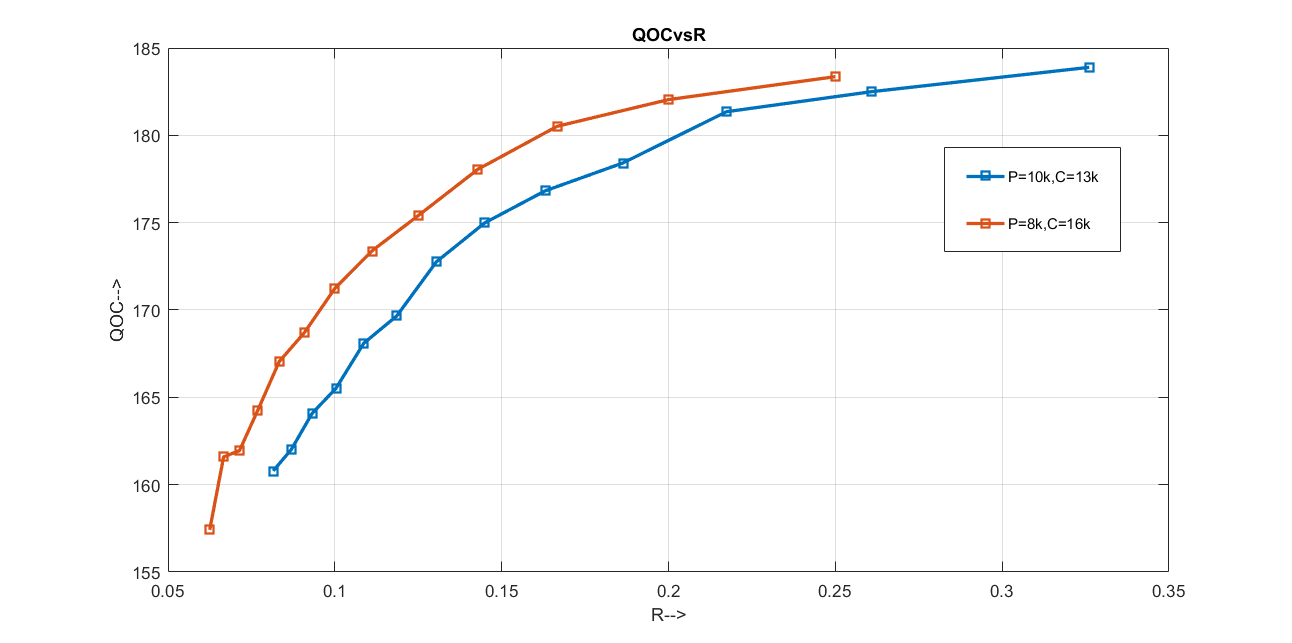
\includegraphics[width=\linewidth]{img/qoc2}
		\caption{QOC vs R for different C and P.}
		\label{fig:qoc2}
	\end{center}
\end{figure}